% -*- TeX-master: "main.tex" -*-

\section{Versuchsdurchführung und Erkenntnisse}
\label{sec:versuch}

Zur veranschaulichung der Ergebnisse werden diese im Folgenden grafisch dargestellt.
Bei der Versuchsdurchführung wird stets ein belieber Graph mit zufälliger Anzahl an Ameisen gewählt. Jeder Takt (step) wird in einem Bild veranschaulicht.\par
Zur Visualisierung ist jeder Knoten mit einem eindeutigen Namen versehen.
Dazu werden links die Anzahl der suchenden und rechts die der heimkehrenden Ameisen abgedruckt.
Die Zahl auf einer Kante ist die dazugehörige Pheromonspur.

\subsection{Versuch 1}
Abbildung \ref{fig:v1} stellt einen Graphen mit 20 Knoten und elf Blattknoten dar. Initial sitzen 6 Ameisen auf dem Startknoten.

\begin{figure}[htbp]
	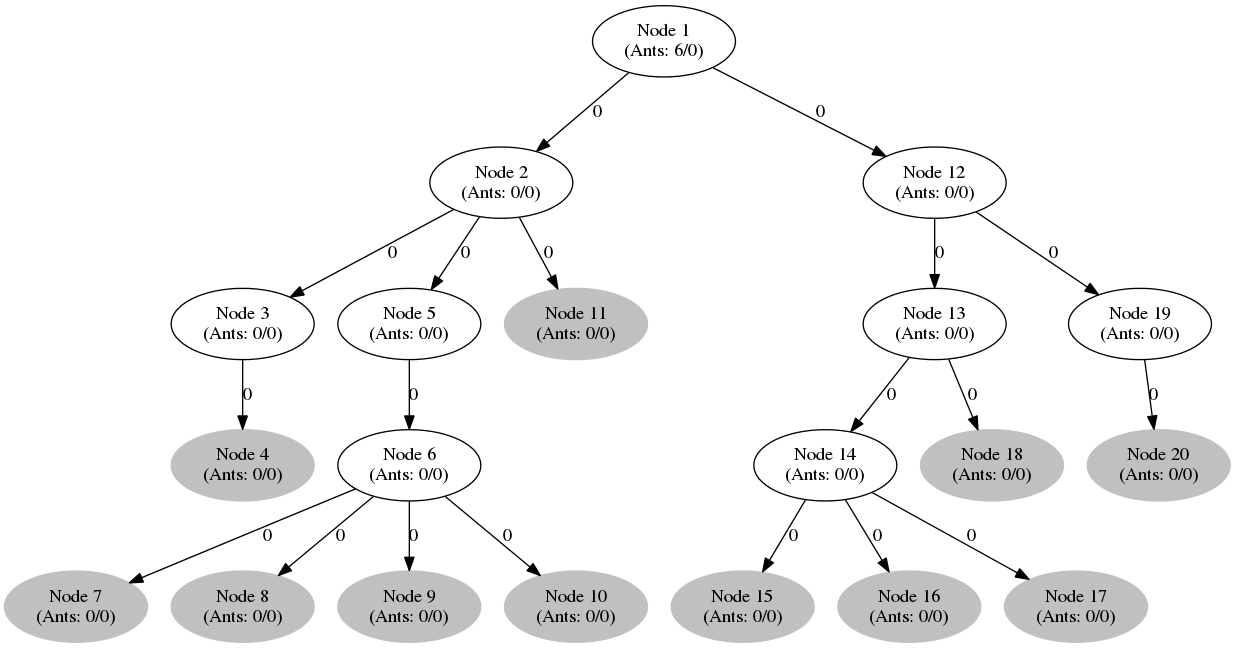
\includegraphics[width=.9\textwidth]{images/v1_1.png}
	\caption{Startzustand Versuch 1.}
	\label{fig:v1}
\end{figure}

Betrachten wir alle Blattknoten (grau) als äquivalente Futterquellen, so ist offensichlicht der Weg über \emph{Node 2} zu \emph{Node 11} der Kürzeste.

\begin{figure}[htbp]
	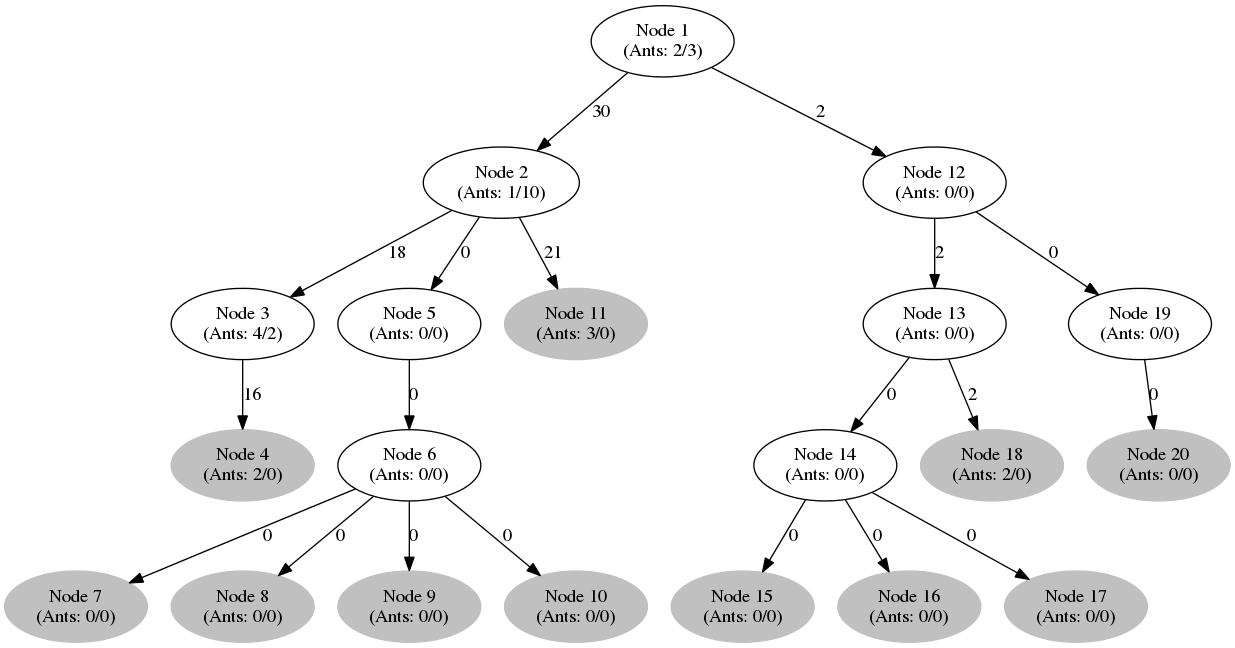
\includegraphics[width=.9\textwidth]{images/v1_6.png}
	\caption{Versuch 1 zu Takt 6.}
	\label{fig:v1_6}
\end{figure}

Wie Abbildung \ref{fig:v1_6} zeigt ist in Takt 6 der Weg zu Node 11 präferiert.
Dieser Zustand ist (vgl. Abbildung \ref{fig:v1_334}) in Takt 334 noch mehr ausgeprägt. Interessant ist hierbei jedoch, dass der Weg zu \emph{Node 18} mit 150 besuchten Ameisen auch stark ins Gewicht fällt. Zufällig ist jedoch der Unterschied zwischen den Verschiedenen Pfaden der Länge 4, wie bswp. der zu \emph{Node 20}.
\begin{figure}[htbp]
	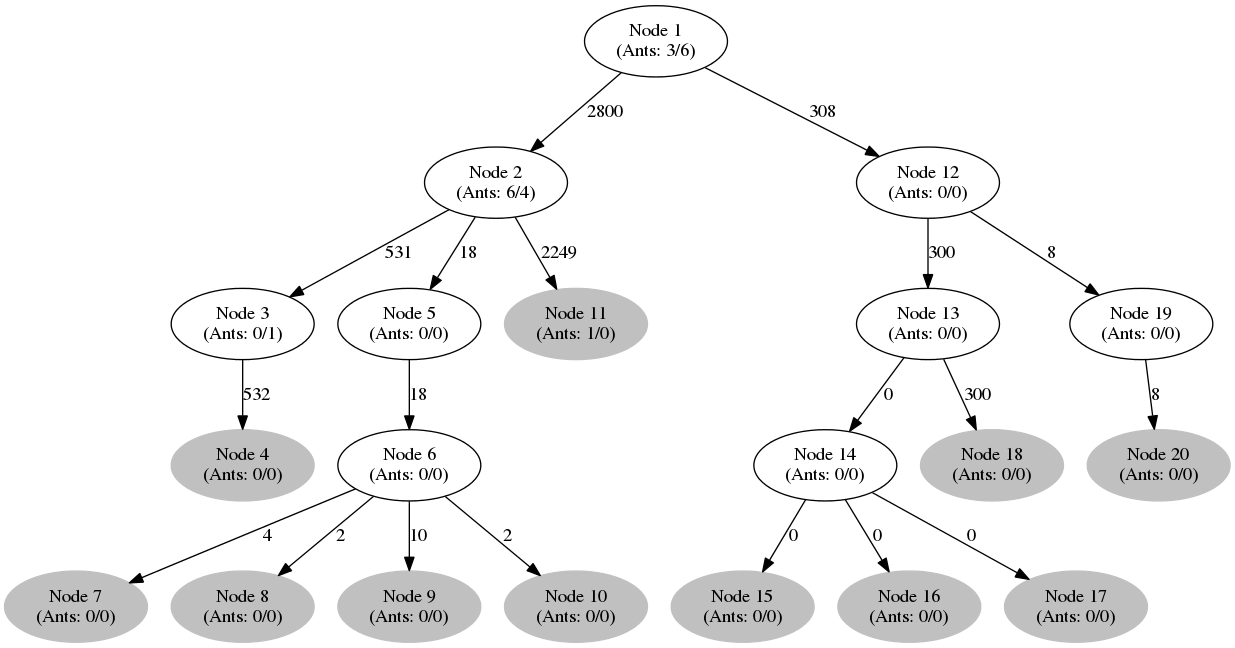
\includegraphics[width=.9\textwidth]{images/v1_334.png}
	\caption{Versuch 1 zu Takt 334.}
	\label{fig:v1_334}
\end{figure}
Trotz dieser Streuungen ist die Präferenz für den kürzesten Weg in diesem Versuch eindeutig zu erkennen.

\subsection{Versuch 2}
In Versuch 2 wird ein Graph mit 26 Knoten, davon 16 Blattknoten, untersucht.
Interessant ist hierbei, dass es mit den Pfaden zu Node 18, 19 und 26 drei äuqivalente kürzeste Pfade gibt.\par
In Takt 3 (Abbildung \ref{fig:v2_3}) sieht man eine gleichmäßige Verteilung der Ameisen auf die verschiedenen Knoten der dritten Stufe. 

\begin{figure}[htbp]
	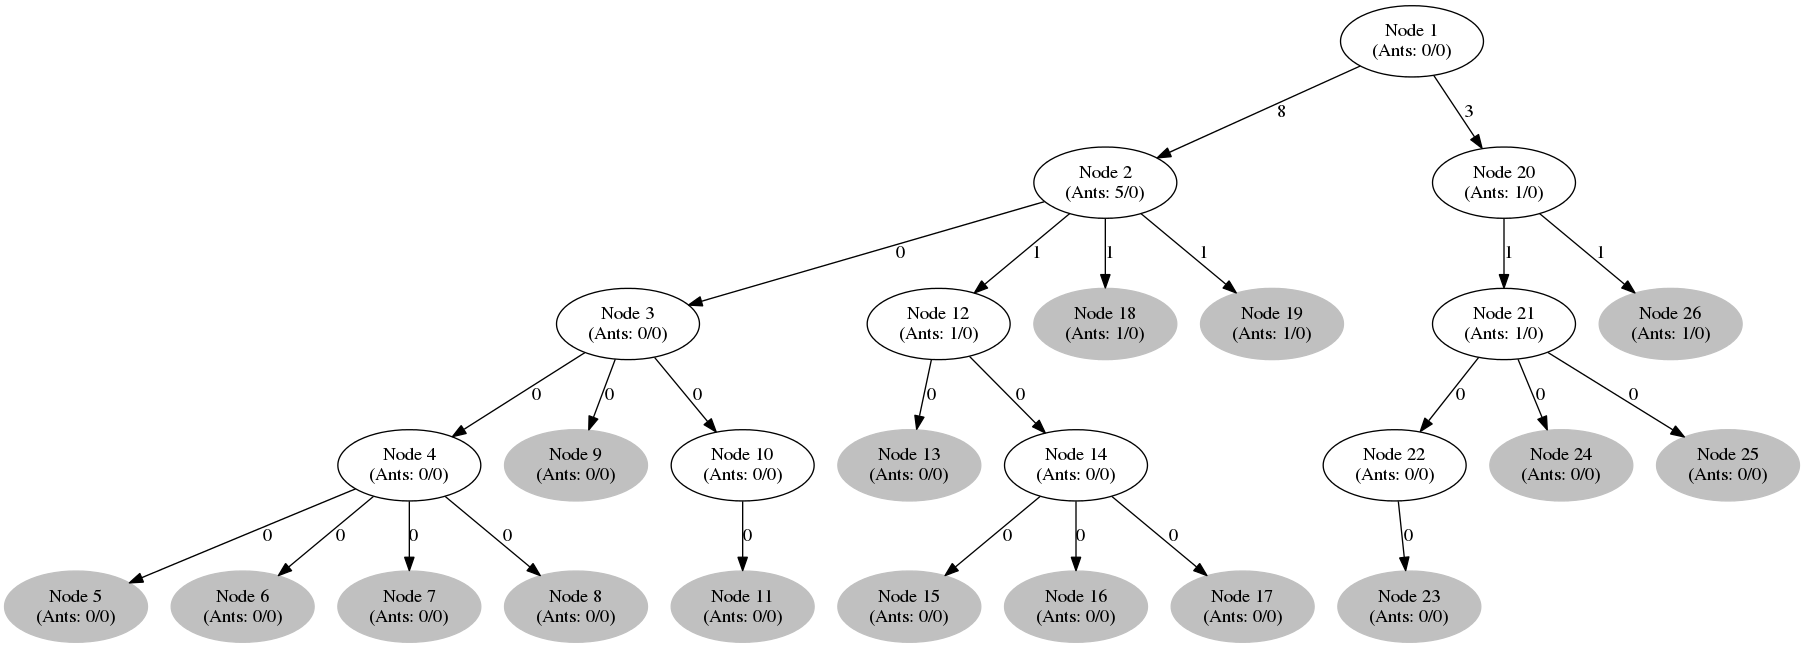
\includegraphics[width=.9\textwidth]{images/v2_3.png}
	\caption{Versuch 2 zu Takt 3.}
	\label{fig:v2_3}
\end{figure}

Durch zufällige Verteilung der weiteren Ameisen kommt es in Takt 7 (Abbildung \ref{fig:v2_7}) zu einer Häufung von \emph{Node 19}.

\begin{figure}[htbp]
	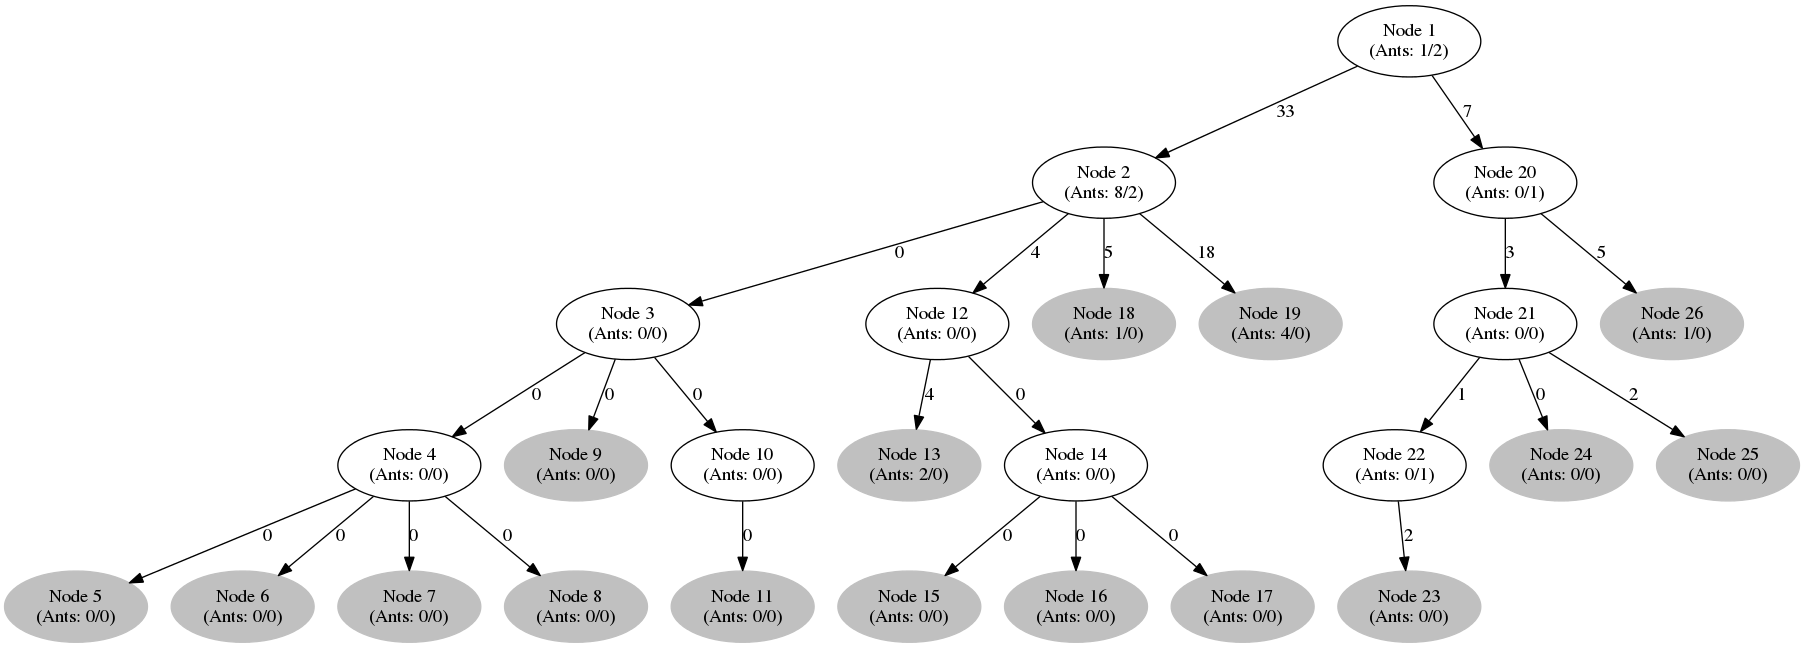
\includegraphics[width=.9\textwidth]{images/v2_7.png}
	\caption{Versuch 2 zu Takt 7.}
	\label{fig:v2_7}
\end{figure}

Diese Ausprägung verstärkt sich nun immer mehr bis wir in Takt 200 zu Abbildung \ref{fig:v2_200} kommen.

\begin{figure}[htbp]
	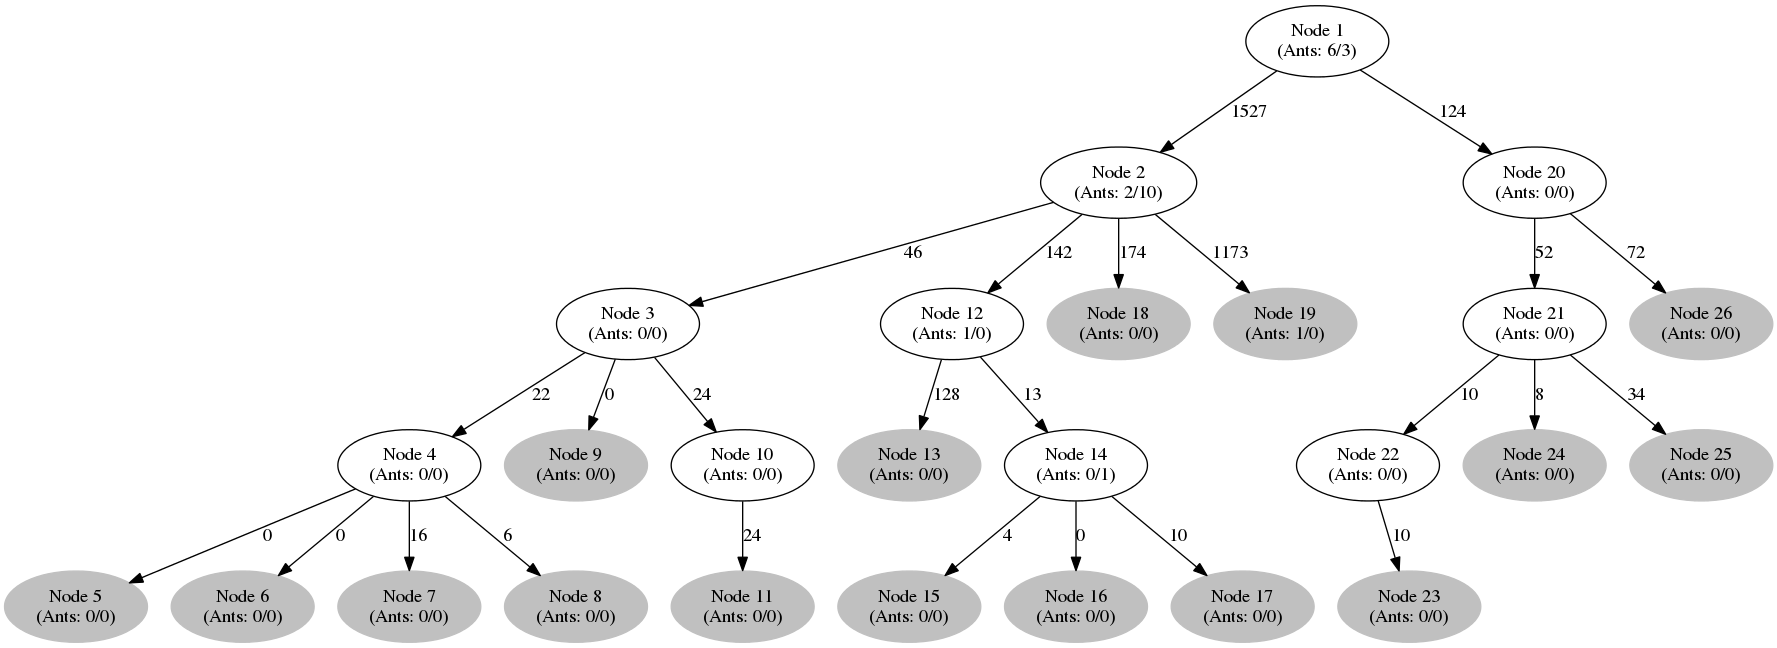
\includegraphics[width=.9\textwidth]{images/v2_200.png}
	\caption{Versuch 2 zu Takt 200.}
	\label{fig:v2_200}
\end{figure}

Interessant ist hier vor allem der Unterschied zwischen den äquivalenten kürzesten Pfaden. Dieser kann durch die Zufallsverteilung erklärt werden.
Wie in Versuch 1 ist jedoch hier wieder der präferierte ein kürzester Weg.

\subsection{Versuch 3}
Versuch 3 ähnelt sehr stark den Versuchen 1 und 2 und ist somit nur kurz zu Takt 1002 in Abbildung \ref{fig:v3_1002} dargestellt.

\begin{figure}[htbp]
	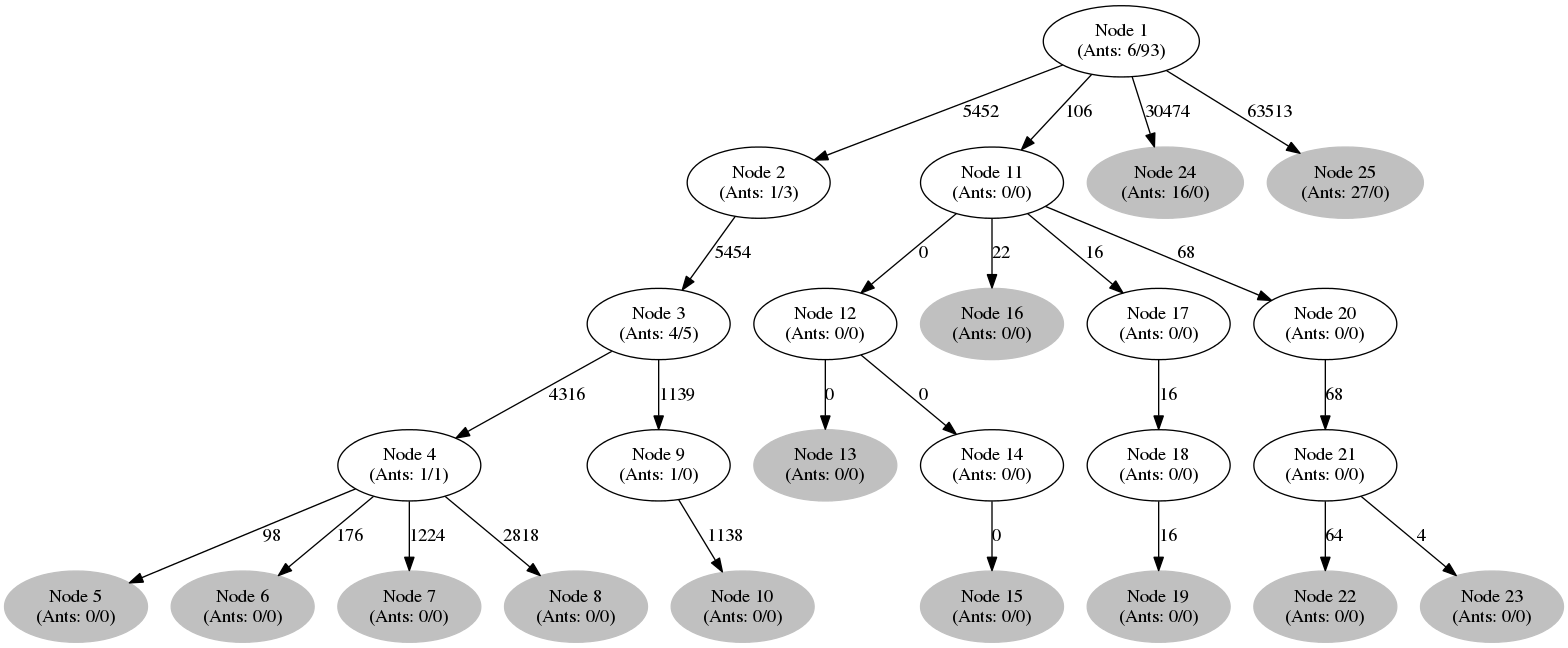
\includegraphics[width=.9\textwidth]{images/v3_1002.png}
	\caption{Versuch 3 zu Takt 1002.}
	\label{fig:v3_1002}
\end{figure}

Hierbei sind wieder die beiden kürzesten Wege zu \emph{Node 24} und \emph{Node 25} die ausgeprägtesten.


\subsection{Versuch 4}
Versuch 4 unterschiedet sich vor allem in der einfacheren Struktur von den bisher aufgeführten Graphen. Da sich die Ameisen hierbei gleich wie bei den bisherigen Versuchen verhalten, betrachten wir wieder einen Takt in Abbildung \ref{fig:v4_334}.

\begin{figure}[htbp]
	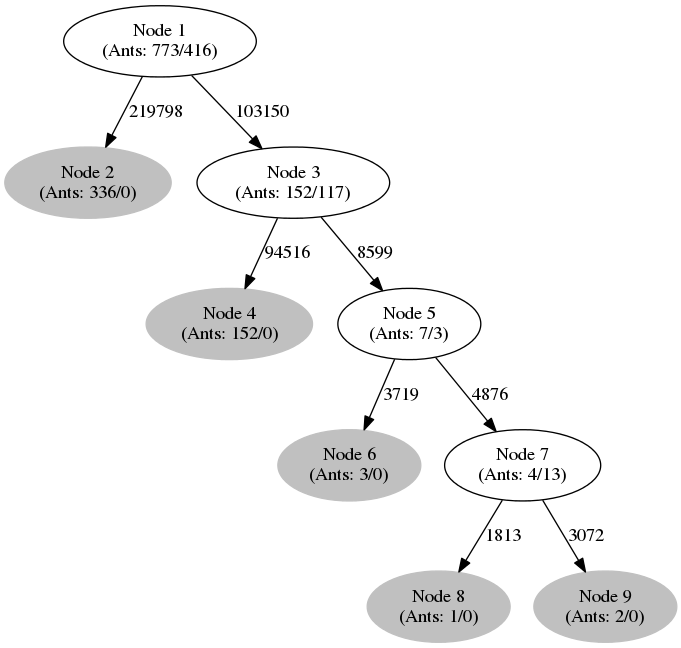
\includegraphics[width=.5\textwidth]{images/v4_334.png}
	\caption{Versuch 4 zu Takt 334.}
	\label{fig:v4_334}
\end{figure}

Bei diesem Versuch sieht man auch offensichtlich, was die Länge des Weges für einen Einfluss auf die Pheromonspur hat.

\subsection{Versuch 5}
Abbildung \ref{fig:v5_2} zeigt den Graphen in Takt 2. Die Struktur des Graphen ähnelt wieder der der anderen Versuche.
Interessant ist hierbei, dass pro Takt zwischen 0 und 1000 Ameisen auf den Startpunkt gesetzt werden. Deshalb kommt es ab Takt 2 zu einem entscheidenden Fehler: Die beiden kürzesten Wege werden nicht mehr berücksichtigt.

\begin{figure}[htbp]
	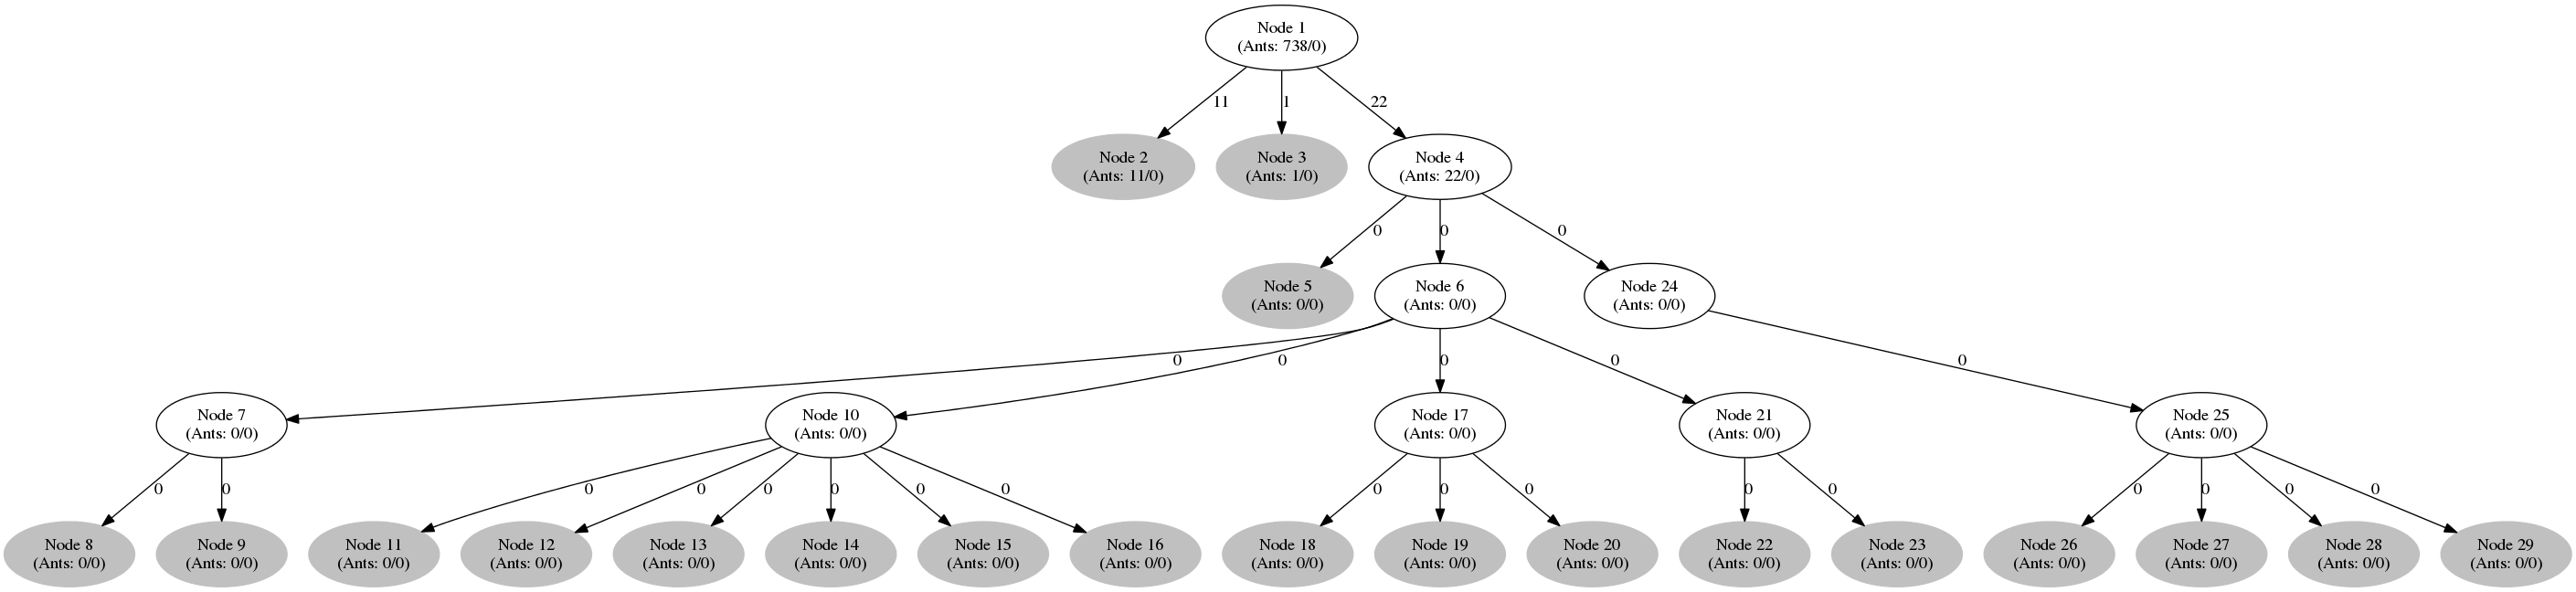
\includegraphics[width=\textwidth]{images/v5_2.png}
	\caption{Versuch 5 zu Takt 2.}
	\label{fig:v5_2}
\end{figure}

Diese "`Fehlentscheidung"' ist zu dem späteren Takt 531 (Abbildung \ref{fig:v5_531}) noch ausgeprägter.

\begin{figure}[htbp]
	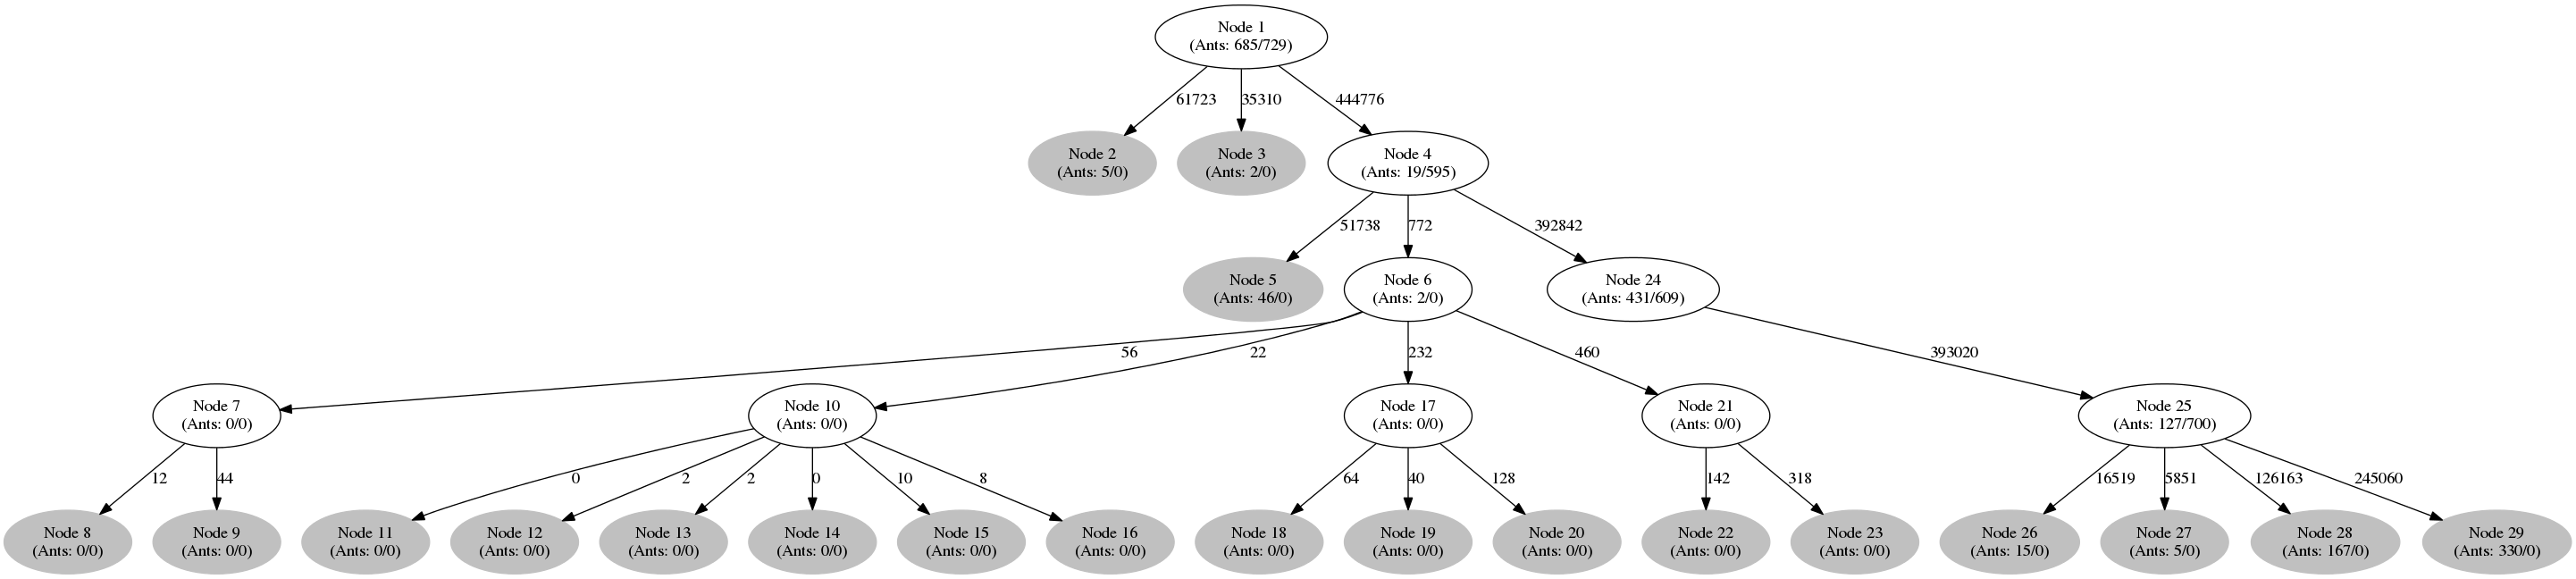
\includegraphics[width=\textwidth]{images/v5_531.png}
	\caption{Versuch 5 zu Takt 531.}
	\label{fig:v5_531}
\end{figure}

Der präferierteste Weg zu \emph{Node 29} ist einer der Längsten. 
Dieser Versuch zeigt uns klar, dass das anfängliche "`blinde"' Suchen der Ameisen  nur bis zu einer geringen Menge an parallel suchender Ameisen funktioniert, da sonst diese Zufälligkeit leicht die früher heimkehrenden Ameisen übertrifft.

\subsection{Erkenntnisse}
\label{sec:erkent}
Wie wir in den Versuchen 1 bis 4 deutlich gesehen haben, funktioniert der Algorithmus für beliebig komplexe Problematiken gut.
Aufgrund der anfänglich rein zufälligen Auswahl der Wege ist es jedoch nicht möglich eine größere Anzahl von Ameisen auf einmal loszuschicken (vgl Versuch 5).
Würde man diese reine Zufälligkeit mit etwas Heuristik ausbauen, würden der Algorithmus jedoch auch größere Mengen Ameisen zum gewünschten Ziel führen.
Aufgrund der Komplexität haben wir jedoch bei unseren Durchführung darauf verzichtet.\par 
Offensichtlich, jedoch nicht an einem Beispiel gezeigt, ist, dass die Situation wie sie in Versuch 5 aufgetreten ist auch in jedem anderen Graphen hätte auftreten können. Jedoch haben wir auch hier aufgrund der großen Komplexität darauf verzichtet, mehrere Durchläufe mit dem gleichen Graphen zu protokollieren.

% - anfängliche heuristik
% - pheromone verschwinden??
% - mehrere Durchläufe mit dem gleichen Graph!